\documentclass[paper=a4, landscape, DIV9, 9pt, abstracton, headings=normal,
						captions=tableheading]{scrartcl}
\usepackage[T1]{fontenc}
\usepackage[utf8]{inputenc}
\usepackage[english,german,ngerman]{babel}
\usepackage[german]{keystroke}
\usepackage{graphicx}
\usepackage{booktabs}
\usepackage{url}
\usepackage{kpfonts}
\usepackage{microtype}
\usepackage{tikz}
\usetikzlibrary{shapes.geometric,shapes.misc,arrows,matrix,fadings,calc,%
		positioning,decorations.pathreplacing,decorations.text,fit}
\newcommand{\cmd}[1]{{\ttfamily#1}}
\newcommand{\incscr}[1]{\includegraphics[scale=0.5]{#1}}
\newcommand{\btngreen}{grün}
\definecolor{btngreen}{rgb}{0.0,0.6,0.0}
\definecolor{btnblue}{rgb}{0.0,0.3,0.6}
\definecolor{btnred}{rgb}{0.6,0.0,0.0}
\newcommand{\bluepairhoriz}[2]{
	\draw[->,thick,btnblue] ($(#1.east)+(0,0.1)$) --
		($(#2.west)+(0,0.1)$) node [midway,above] {rechts};
	\draw[<-,thick,btnblue] ($(#1.east)+(0,-0.1)$) --
		($(#2.west)+(0,-0.1)$) node [midway,below] {links};
}
\newcommand{\greeneditfromto}[2]{
	\draw[->,thick,btngreen] ($(#1.south)+(-0.2,0.0)$) --
		($(#2.north)+(-0.2,0.0)$) node [midway,left] {\btngreen};
	\draw[<-,thick,btngreen] ($(#1.south)+(0.2,0.0)$) --
		($(#2.north)+(0.2,0.0)$) node [midway,right] {\btngreen};
	\draw[<->,thick,btnblue] (#2) edge[loop below,looseness=2.5] (#2)
				node[below,yshift=-0.9cm] {verstellen};
	% alt: kleiner/größer
}
% https://tex.stackexchange.com/questions/18200/draw-edges-and-paths-in-the-
\pgfdeclarelayer{bg}
\pgfsetlayers{bg,main}
\begin{document}
\thispagestyle{empty}
\begin{tikzpicture}[remember picture,overlay]
	\tikzset{scr/.style={fill=white,draw}}
	\node[anchor=north west,xshift=2.5cm,yshift=-1.5cm] at
				(current page.north west) (anchor) {~};

	\node[below=1cm of anchor,scr]     (scrstart)   {\incscr{scrstart}};
	\node[right=1cm of scrstart,scr]   (scrstartal) {\incscr{scrstartal}};

	\node[below=1cm of scrstart,scr]   (scralm1)    {\incscr{scralm1}};
	\node[right=1cm of scralm1,scr]    (scralm2)    {\incscr{scralm2}};
	\node[right=1cm of scralm2,scr]    (scralm3)    {\incscr{scralm3}};

	\node[below=1cm of scralm1]        (startsep)   {\incscr{spacer}};
	\node[below=1cm of scralm2,scr]    (scralm2b)   {\incscr{scralm2b}};
	\node[below=1cm of scralm3,scr]    (scralm3b)   {\incscr{scralm3b}};

	\node[below=1cm of startsep,scr]   (scrdate1)   {\incscr{scrdate1}};
	\node[right=1cm of scrdate1,scr]   (scrdate2)   {\incscr{scrdate2}};
	\node[right=1cm of scrdate2,scr]   (scrdate3)   {\incscr{scrdate3}};
	\node[right=1cm of scrdate3,scr]   (scrdate4)   {\incscr{scrdate4}};
	\node[right=1cm of scrdate4,scr]   (scrdate5)   {\incscr{scrdate5}};
	\node[right=1cm of scrdate5,scr]   (scrdate6)   {\incscr{scrdate6}};
	\node[right=1cm of scrdate6,scr]   (scrdate7)   {\incscr{scrdate7}};
	\node[right=1cm of scrdate7,scr]   (scrdate8)   {\incscr{scrdate8}};

	\node[below=1cm of scrdate1]       (scrsep2)    {\incscr{spacer}};
	\node[below=1cm of scrdate2,scr]   (scrdate2b)  {\incscr{scrdate2b}};
	\node[below=1cm of scrdate3,scr]   (scrdate3b)  {\incscr{scrdate3b}};
	\node[below=1cm of scrdate4,scr]   (scrdate4b)  {\incscr{scrdate4b}};
	\node[below=1cm of scrdate5,scr]   (scrdate5b)  {\incscr{scrdate5b}};
	\node[below=1cm of scrdate6,scr]   (scrdate6b)  {\incscr{scrdate6b}};
	\node[below=1cm of scrdate7,scr]   (scrdate7b)  {\incscr{scrdate7b}};
	\node[below=1cm of scrdate8,scr]   (scrdate8b)  {\incscr{scrdate8b}};

	\node[below=1cm of scrsep2,scr]    (scrinfo1)   {\incscr{scrinfo1}};
	\node[right=1cm of scrinfo1,scr]   (scrinfo2)   {\incscr{scrinfo2}};
	\node[right=1cm of scrinfo2,scr]   (scrinfo3)   {\incscr{scrinfo3}};
	\node[right=1cm of scrinfo3,scr]   (scrinfo4)   {\incscr{scrinfo4}};
	\node[right=1cm of scrinfo4,scr]   (scrinfo5)   {\incscr{scrinfo5}};
	\node[right=1cm of scrinfo5,scr]   (scrinfo6)   {\incscr{scrinfo6}};

	\node[below=1cm of scrinfo1,scr]   (scrver1)    {\incscr{scrversion1}};
	\node[right=1cm of scrver1,scr]    (scrver2)    {\incscr{scrversion2}};
	\node[right=1cm of scrver2,scr]    (scrver3)    {\incscr{scrversion3}};

	\draw[->,thick,btnred] ($(scrstart.east)+(0,0.1)$) --
		($(scrstartal.west)+(0,0.1)$) node [midway,above] {Al.ein};
	\path (scrstart.east) -- (scrstartal.west)
		node [midway,above,yshift=4mm] {$\epsilon$};
	\draw[<-,thick,btnred] ($(scrstart.east)+(0,-0.1)$) --
		($(scrstartal.west)+(0,-0.1)$) node [midway,below] {Al.aus};
	\draw[<-,thick,btngreen] (scrstart) -- +(-2,0) node (scrstartpre) {};

	\draw[->,thick,btngreen] (scrstartal) -- (scralm1)
					node [midway,right] {\btngreen};
	\draw[->,thick,btngreen] (scrstart) -- (scralm1)
					node [midway,left] {\btngreen};
	\draw[->,thick,btnblue] (scralm1) -- +(-2,0)
					node [midway,above] {\small links};
	\draw[->,thick,btngreen] (scralm1) -- (scrdate1)
					node [midway,left] {\btngreen};
	\draw[->,thick,btnblue] (scrdate1) -- +(-2,0)
					node [midway,above] {\small links};
	\draw[->,thick,btngreen] (scrdate1) -- (scrinfo1)
					node [midway,left] {\btngreen};
	\draw[->,thick,btngreen] (scrinfo1) -- (scrver1)
					node [midway,left] {\btngreen};
	\draw[->,thick,btnblue] (scrinfo1) -- +(-2,0)
					node [midway,above] {\small links};
	\draw[->,thick,btnblue] (scrver1) -- +(-2,0)
					node [midway,above] {\small links};

	\bluepairhoriz{scralm1}{scralm2}
	\bluepairhoriz{scralm2}{scralm3}
	\greeneditfromto{scralm2}{scralm2b}
	\greeneditfromto{scralm3}{scralm3b}
	\draw[<-,thick,btnblue] (scrstart) -- +(0,1.5) node (startanch) {};
	\draw[thick,btnblue] (scralm3) -- +(2,0) node (scralm3end) {};
	\path[btnblue] (scralm3) -- +(2,0) node[midway,above] {\small rechts};
	\draw[thick,btnblue] (scralm3end.center) --
			(scralm3end.center|-startanch.center)
			node (retpathinterm1) {} --
			(startanch.center) node [midway,above] {rechts/zurück};

	\bluepairhoriz{scrdate1}{scrdate2}
	\bluepairhoriz{scrdate2}{scrdate3}
	\bluepairhoriz{scrdate3}{scrdate4}
	\bluepairhoriz{scrdate4}{scrdate5}
	\bluepairhoriz{scrdate5}{scrdate6}
	\bluepairhoriz{scrdate6}{scrdate7}
	\bluepairhoriz{scrdate7}{scrdate8}
	\greeneditfromto{scrdate2}{scrdate2b}
	\greeneditfromto{scrdate3}{scrdate3b}
	\greeneditfromto{scrdate4}{scrdate4b}
	\greeneditfromto{scrdate5}{scrdate5b}
	\greeneditfromto{scrdate6}{scrdate6b}
	\greeneditfromto{scrdate7}{scrdate7b}
	\greeneditfromto{scrdate8}{scrdate8b}
	\draw[thick,btnblue] (scrdate8) -- +(2,0) node (scrdate8end) {};
	\path[btnblue] (scrdate8) -- +(2,0) node [midway,above] {\small rechts};
	\draw[->,thick,btnblue] (scrdate8end.center) --
		(scrdate8end.center|-retpathinterm1.center) --
		(retpathinterm1.center) node [midway,above] {rechts/zurück};

	\draw[thick,btnblue] (scrinfo6) -- (scrdate8end.center|-scrinfo6)
			node (scrinfo6end) {};
	\path[btnblue] (scrinfo6) -- (scrdate8end.center|-scrinfo6)
			node [midway,below] {rechts};
	\draw[->,thick,btnblue] (scrinfo6end.center) -- (scrdate8end.center);

	\bluepairhoriz{scrinfo1}{scrinfo2}
	\bluepairhoriz{scrinfo2}{scrinfo3}
	\bluepairhoriz{scrinfo3}{scrinfo4}
	\bluepairhoriz{scrinfo4}{scrinfo5}

	\draw[->,thick,btnblue,align=center] ($(scrinfo5.east)+(0,0.1)$) --
		($(scrinfo6.west)+(0,0.1)$) node [midway,above]
						{$\epsilon$\\[-0.3em] rechts};
	\draw[<-,thick,btnblue,align=center] ($(scrinfo5.east)+(0,-0.1)$) --
		($(scrinfo6.west)+(0,-0.1)$) node [midway,below]
						{links\\[-0.3em] $\epsilon$};

	\bluepairhoriz{scrver1}{scrver2}
	\bluepairhoriz{scrver2}{scrver3}
	\draw[thick,btnblue] (scrver3) -- (scrinfo6end.center|-scrver3)
			node (scrver3end) {};
	\path[btnblue] (scrver3) -- (scrinfo6end.center|-scrver3)
			node [midway,above] {rechts};
	\draw[->,thick,btnblue] (scrver3end.center) -- (scrinfo6end.center);
	\draw[thick,btngreen] (scrinfo2) -- +(0,-1.2) node (scrinfo2bot) {};
	\path[btngreen] (scrinfo2) -- +(0,-1.2) node[midway,right] {\btngreen};
	\draw[->,thick,btngreen] (scrinfo3) -- +(0,-1.2) node[midway,right]
								{\btngreen};
	\draw[->,thick,btngreen] (scrinfo4) -- +(0,-1.2) node[midway,right]
								{\btngreen};
	\draw[->,thick,btngreen] (scrinfo5) -- +(0,-1.2) node[midway,right]
								{\btngreen};
	\draw[->,thick,btngreen] (scrinfo6) -- +(0,-1.2) node[midway,right]
								{\btngreen};
	\draw[->,thick,btngreen] (scrinfo2bot.center) --
			(scrinfo6end.center|-scrinfo2bot) node (scrinfo2end) {};
	\draw[thick,btngreen] (scrver1) -- +(0,-1.5) node (scrver1bot) {};
	\draw[thick,btngreen] (scrver2) -- +(0,-1.5) node (scrver2bot) {};
	\draw[->,thick,btngreen] (scrver2bot.center) -- (scrver1bot.center)
			node [midway,above] {\btngreen};
	\draw[thick,btngreen] (scrver3) -- +(0,-1.5) node (scrver3bot) {};
	\draw[->,thick,btngreen] (scrver3bot.center) -- (scrver2bot.center)
			node [midway,above] {\btngreen};

	\draw[thick,btngreen] (scrstartpre.center) --
			(scrstartpre.center|-scrver1bot.center) --
			(scrver1bot.center) node [midway,above] {\btngreen};

	\node[right=2cm of scralm3] (picsmall)
				{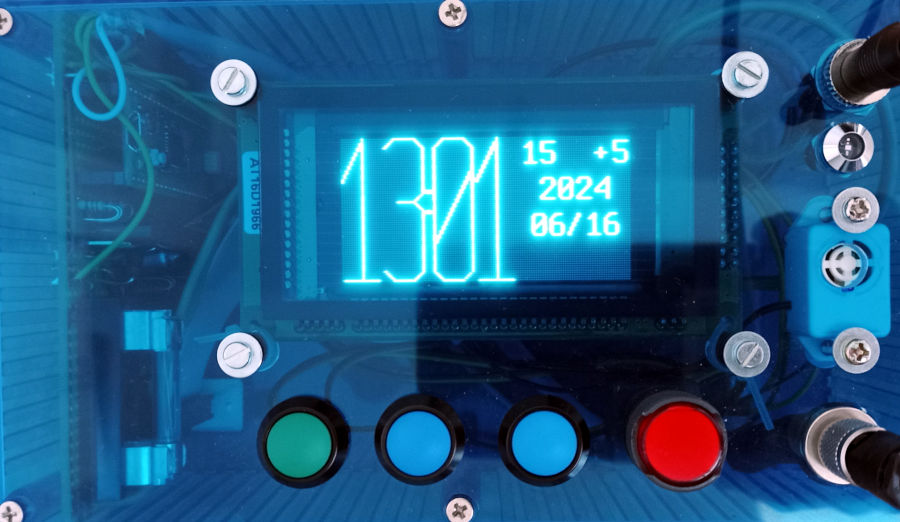
\includegraphics[height=7cm]{picsmall}};
	\path (picsmall.center) -- +(-2.2,-2.3) node (lblgreen)
			{\color{white}\colorbox{btngreen}{\textbf{\btngreen}}};
	\node[right=0.5cm of lblgreen] (lblleft)
			{\color{white}\colorbox{btnblue}{\textbf{links}}};
	\node[right=0.5cm of lblleft] (lblright)
			{\color{white}\colorbox{btnblue}{\textbf{rechts}}};
	\node[right=0.5cm of lblright] (lblalarm)
			{\color{white}\colorbox{btnred}{\textbf{Wecker}}};

	\path (picsmall.center) -- +(4.4,1.5) node (lblals)
			{\colorbox{white}{\textbf{Lichtsensor}}};
	\node[below=1cm of lblals] (lblbuzz)
			{\colorbox{white}{\textbf{Buzzer}}};
	\path (picsmall.south east) -- +(-0.5,1) node (lblant)
			{\colorbox{white}{\textbf{Antennenanschluss}}};
	\node[above=4.5cm of lblant] (lblpwr)
			{\colorbox{white}{\textbf{5V-Stromversorgung}}};

	\node[above=3cm of lblgreen,xshift=-1cm] (lbltime)
			{\colorbox{white}{\textbf{Uhrzeit Stunde:Minute}}};
	\node[above=1cm of lblright,xshift=0.5cm] (lbldate)
			{\colorbox{white}{\parbox{1.7cm}{%
			\bfseries Datum Jahr\newline Monat/Tag}}};
	\node[left=2cm of lblpwr,yshift=-0.5cm] (lblseconds) {%
			\colorbox{white}{\parbox{1.3cm}{%
			\textbf{Uhrzeit Sekunde}}}};
	\node[above=0.2cm of lblseconds,xshift=1.5cm] (lblqos)
			{\colorbox{white}{\textbf{Signalqualität}}};

	\node[right=0.3cm of lblseconds.south east] (qosanchor) {};
	\draw[thick,white,->] ($(lblqos.south)+(0,+0.2)$) -- (qosanchor);

	\path (scrinfo6.center) -- +(5.7,-4) node[draw] (lblplankopf)
		{\begin{minipage}{6cm}\begin{center}
		Ma\_Sys.ma DCF77 VFD Raspi Clock\\
		Bedienung und Übersicht der Anzeigezustände\\
		2025-01-05 \qquad \cmd{info@masysma.net}
		\end{center}\end{minipage}};

	\begin{pgfonlayer}{bg}
		\node[inner sep=3mm,fill=black!10,fit=(scrstartal) (scralm3b)]
				(areaalm) {};
		\node[inner sep=3mm,fill=black!10,fit=(scrdate2) (scrdate8b)]
				(areadate) {};
		\node[inner sep=3mm,fill=black!10,fit=(scrinfo6) (scrver1)]
				(areaextra) {};
	\end{pgfonlayer}

	\node[above=1cm of scralm3,text width=2cm,xshift=-0.5cm]
			(lblareaalm) {\textbf{\huge Wecker-\\einstellung}};
	\node[below=0.7cm of scrdate8b,xshift=-0.92cm,fill=black!10]
			(lblareadate) {\textbf{\huge Datumseinstellung}};
	\node[right=5.5cm of scrver3,text width=5cm,yshift=-0.5cm]
			(lblareaextra) {\textbf{\huge{Statusinformationen}}};

	\begin{pgfonlayer}{bg}
		\node[inner sep=1mm,fill=black!10,fit=(scrdate8) (lblareadate)]
				(areadate2) {};
	\end{pgfonlayer}
\end{tikzpicture}
\end{document}
